\chapter{Tecnologie e strumenti}
\section{Introduzione}
In questo capitolo, verranno descritti i tool, le tecnologie e i framework utilizzati per lo sviluppo del progetto, proponendo le considerazioni che hanno portato alla loro scelta rispetto alle principali alternative, che verranno descritte anch'esse per fornire una panoramica della strumentazione software disponibile indipendentemente dal progetto argomento di questa tesi.
Il focus sarà sulle tecnologie dell'ambiente Microsoft \emph{.NET}, mentre i tool di contorno sono stati o saranno brevemente descritti quando menzionati.

\section{Panoramica del framework}
È anzitutto necessari fare distinzione tra \emph{.NET Framework} e \emph{.NET}: il primo è la versione originale di .NET, rilasciata nel 2002 e tuttora supportata, ma limitata alla sola piattaforma Windows e non più in fase di sviluppo attivo, mentre il secondo è una riscrittura completa del framework, nata nel 2016 come .NET Core per poi evolversi nell'attuale .NET 5+ a partire dal 2020, che è open source, multipiattaforma (Windows, Linux, macOS) e in continua evoluzione con nuove funzionalità e miglioramenti delle performance. Per il resto del testo, faremo riferimento a .NET 5+ (d'ora in poi indicato semplicemente come \textbf{.NET}).

Microsoft .NET è un framework di sviluppo open source e multiplatform, che consente lo sviluppo rapido e produttivo di software moderno e performante in una nutrita varietà di ambiti, dallo sviluppo web, cloud, desktop e mobile fino al gaming, all'IoT e al Machine Learning.
Il cuore della piattaforma è il \textbf{Common Language Runtime (CLR)}, l'engine di esecuzione, a cui sono affidati tutti gli aspetti legati alla gestione della memoria (e.g. \emph{Garbage Collection}), della sicurezza, della gestione delle eccezioni e del multithreading.

Come comportamento predefinito, il codice sorgente dei linguaggi .NET è compilato in un linguaggio intermedio e \emph{platform-independent}, chiamato appunto \textbf{Intermediate Language (IL)}. Il risultato di una build è un file eseguibile, detto \textbf{assembly}, il quale contiene il codice IL, i metadati, le dipendenze, e può opzionalmente essere \emph{self-contained} (ossia include il runtime necessario all'esecuzione). All'utilizzo (avvio dell'eseguibile o invocazione della dll), sarà il \textbf{CLR} a effettuare una compilazione \emph{Just In Time (JIT)} del codice IL in codice macchina nativo, specifico e ottimizzato per l'architettura hardware della macchina che ospita l'esecuzione.

È altresì possibile configurare il compilatore per ottenere un comportamento \emph{Ahead Of Time (AOT)}, in cui il codice IL viene compilato in codice macchina nativo al momento della build, migliorando i tempi di avvio dell'applicazione e riducendo il consumo di memoria: tale alternativa tuttavia inficia sulla portabilità e rinuncia a ottimizzazioni specifiche per l'architettura hardware che sarebbero invece possibili con la compilazione \emph{JIT}.

.NET supporta offre tre linguaggi di programmazione nativi: C\#, F\# e Visual Basic, ma grazie alla presenza del \textbf{Common Type System (CTS)} e del \textbf{Common Language Specification (CLS)}, è possibile utilizzare anche altri linguaggi compatibili, come ad esempio C++/CLI, Python o Ruby.

C\# è il linguaggio più diffuso: si tratta di un linguaggio di programmazione \emph{type-safe}, orientato agli oggetti, con una sintassi \emph{C-like} (ispirata cioè a linguaggi come C, C++ e Java) moderna che ne facilita l'apprendimento e la produttività.
C\# supporta anche paradigmi di programmazione funzionale, come le espressioni lambda, i delegati e le \emph{LINQ} (\underline{\textbf{L}anguage \textbf{IN}tegrated \textbf{Q}uery}), che permettono di scrivere codice conciso ed espressivo e facilitano la manipolazione di collezioni di dati (per esempio LINQ mette a disposizione una sintassi dichiarativa ispirata a SQL per la manipolazione programmatica integrata delle collezioni di dati).

F\# è un linguaggio di programmazione funzionale dalla sintassi concisa, proprietà che lo rendono ideale per scenari che richiedono un'elaborazione complessa dei dati, come il calcolo scientifico, l'analisi finanziaria e il Machine Learning. L'enfasi sulla programmazione funzionale non esclude un supporto per la programmazione imperativa e quella orientata agli oggetti, tuttavia la sintassi povera di parentesi e annidamenti e le funzionalità del linguaggio pongono il focus sul costruire aggregati operativi potenti piuttosto che "dati con azioni associate".

Visual Basic (VB.NET) è un linguaggio di programmazione ad alto livello, noto per la sua sintassi semplice simile al linguaggio naturale inglese che lo rende accessibile ai principianti. Originariamente sviluppato per la creazione di applicazioni desktop Windows, VB.NET ha visto un declino della popolarità negli ultimi anni, in favore di C\# e F\#. Tuttavia, rimane una scelta valida per progetti legacy o per sviluppatori con esperienza pregressa in Visual Basic.

Per quanto riguarda gli altri linguaggi per cui la piattaforma .NET offre supporto, i metodi di integrazione con il framework variano a seconda del linguaggio, ma si riducono principalmente a due approcci: l'\emph{hosting} su CLR di interpreti o VM per l'esecuzione del codice sorgente, utilizzando \emph{binding} nativi per interfacciarsi con le librerie .NET tramite API specifiche del linguaggio, oppure la compilazione in Intermediate Language (IL) tramite un compilatore dedicato: questa soluzione consente di sfruttare appieno le funzionalità della piattaforma .NET, ma lo sviluppo di un compilatore apposito arriva spesso per linguaggi la cui compatibilità con .NET riceve un supporto maggiore dalla community.

\section{ASP.NET Core}
ASP.NET Core è il framework Microsoft dedicato allo sviluppo di applicazioni e servizi web moderni, scalabili e performanti in ambiente .NET con C\#, con supporto per Windows, Linux, macOS e Docker per il deploy in container \cite{aspdotnet_site}.
Lo scopo di ASP.NET Core è quello di fornire un'infrastruttura robusta, modulare e performante (la cruda potenza di elaborazione dei servizi .NET è provata in numerosi test e benchmark indipendenti \cite{benchmark}) per la creazione di applicazioni web, API RESTful, applicazioni in tempo reale e microservizi.

I vanti del framework sono molteplici. Anzitutto, ASP.NET Core è open source e supportato da una vasta community di sviluppatori, che contribuiscono attivamente al suo sviluppo e alla creazione di librerie e strumenti aggiuntivi, garantendo supporto e strumenti allo sviluppatore.
In un Internet che richiede standard sempre più elevati in termini di sicurezza, ASP.NET Core offre funzionalità integrate per la gestione dell'autenticazione, dell'autorizzazione, della protezione contro attacchi comuni (e.g. CSRF, XSS) e della crittografia dei dati.

Un altro punto di forza è la modularità: il framework è progettato per essere leggero e modulare, consentendo agli sviluppatori di includere solo i componenti necessari per la loro applicazione, riducendo così l'ingombro e migliorando notevolmente le performance.
Questo aspetto risalta con facilità all'interno dei file di configurazione del progetto ASP.NET Core, in cui vengono raccolti i riferimenti alle librerie e ai pacchetti \textbf{NuGet} (\emph{Package Manager} ufficiale .NET) necessari per il funzionamento dell'applicazione, rendendo opzionali tutte le funzionalità del framework non strettamente indispensabili.

La configurazione dei servizi e l'elaborazione delle richieste HTTP in ASP.NET Core sono centralizzate, minimali e dichiarative. Esse avvengono all'interno dell'\emph{entrypoint} dell'applicazione, il file \texttt{Program.cs},
che consta di due sezioni principali. All'inizio del file, si istanzia un \emph{builder} per l'applicazione: tramite esso è possibile aggiungere e configurare i servizi necessari (importati tramite NuGet) all'applicazione, che verranno poi iniettati nei componenti che ne fanno richiesta tramite il meccanismo di \emph{Dependency Injection} (DI) nativo di ASP.NET Core.
Dopo aver configurato i servizi, viene eseguito il \emph{build} dell'applicazione: un oggetto \texttt{app} viene creato a partire dal \texttt{builder}, e rappresenta l'applicazione web vera e propria.
Da questo punto fino al termine del file, contrassegnato dal \texttt{Run()} dell'applicazione, viene definita in maniera \emph{order-sensitive} la pipeline di elaborazione delle richieste HTTP. I servizi configurati abilitano l'utilizzo di \emph{middleware} (in \texttt{Program.cs} rappresentati da metodi invocabili sull'istanza dell'oggetto \texttt{WebApplication}) che intercettano e processano sequenzialmente le richieste in ingresso, e in ordine inverso le risposte in uscita: esempi comuni di middleware sono quelli per la gestione degli errori, del routing, dell'autenticazione e dell'autorizzazione, del logging, della compressione delle risposte.

\begin{lstlisting}[language={[Sharp]C}, caption={[Esempio Program.cs]Esempio di struttura di un file \texttt{Program.cs} in un progetto ASP.NET Core.}, label=lst:programcs]
var builder = WebApplication.CreateBuilder(args);

builder.Services.AddServiceX().SettingA();
builder.Services.AddServiceY(lambdaParam =>
        options.DoSomething()
).SettingB(param1, param2);

var app = builder.Build();

app.UseMiddlewareX();
app.UseMiddlewareY();

app.Run();
\end{lstlisting}
Nelle sezioni successive, verranno descritte le tecnologie e i framework specifici di ASP.NET Core che rappresentano elementi chiave nella realizzazione del progetto di tirocinio e le loro alternative fornite dalla piattaforma.

\section{ASP.NET Core Web API}
È il modello di programmazione web di ASP.NET Core dedicato alla creazione di servizi HTTP RESTful, ossia API che forniscono risorse (solitamente in formati testuali come JSON o XML) e funzionalità a client remoti come app mobile, SPA (Single Page Application) o altri server, il tutto seguendo il paradigma \textbf{REST} descritto nel secondo capitolo. Le API sono progettate per fornire un accesso \emph{programmatico} a un servizio, per cui non restituiscono mai pagine HTML (è il compito del modello MVC analizzato in seguito), ma solo dati e metadati strutturati.
Il framework supporta nativamente la serializzazione e deserializzazione automatica dei dati (come gli oggetti C\#) in formati comuni come JSON e XML, semplificando lo scambio di dati tra client e server. Inoltre, offre funzionalità integrate per la gestione della validazione dei dati, della gestione degli errori, del versioning delle API e della documentazione automatica tramite strumenti come Swagger (anch'esso adottato nel progetto di tirocinio e descritto in seguito).

L'astrazione concettuale del modello ASP.NET Core Web API è la seguente. Seguendo la filosofia REST, le risorse sono identificate da URL univoci e accessibili tramite i verbi HTTP standard (GET, POST, PUT, DELETE, ecc.); ogni URL costituisce un \textbf{endpoint} dell'API, ossia un punto di accesso su cui il client può richiedere una risorsa o un servizio, ed è compito del server ASP.NET Core rispondere a tali richieste. \cite[p.47]{Pro_ASP.NET}
Per implementare l'idea appena descritta, ASP.NET Core fornisce due approcci principali per la definizione degli endpoint di un'API: il modello basato su controller (più maturo e completo) e il modello delle Minimal API (introdotto in .NET 6, più leggero e conciso).

Nel primo modello (quello adottato per la realizzazione del progetto di tirocinio), l'unità di elaborazione logica in ASP.NET Core Web API è il \textbf{controller}: un controller è una classe C\# definita dal programmatore che eredita dalla classe \texttt{ControllerBase} e incapsula la logica di gestione delle richieste e delle risposte per uno o più endpoint specifici.
Un controller espone metodi pubblici (detti \emph{action method}) per definire la logica di elaborazione e risposta alle richieste HTTP su un certo endpoint; ogni controller è annotato con un \emph{attributo} di routing (e.g. \texttt{[Route("[controller]")]}) che specifica l'URL di base per gli endpoint sotto la sua responsabilità, mentre i metodi sono marcati con attributi che indicano il verbo HTTP supportato e il percorso relativo dell'endpoint rispetto all'URL base del controller (e.g. \texttt{[HttpGet(Name = "NomeRisorsa")]}).

Il secondo modello, quello basato su \emph{Minimal API}, consente di definire gli endpoint direttamente nel file \texttt{Program.cs} dell'applicazione, senza la necessità di creare controller separati. Questo approccio è più conciso e adatto per API semplici o microservizi, ma può risultare meno organizzato e manutenibile per applicazioni più complesse.
L'idea è in buona sostanza quella di definire gli endpoint all'interno di metodi middleware nella pipeline di elaborazione delle richieste, utilizzando metodi come \texttt{MapGet}, \texttt{MapPost}, \texttt{MapPut} e \texttt{MapDelete} per associare un URL e un verbo HTTP a una funzione lambda o un altro tipo di funzione di ordine superiore che implementa la logica di gestione della richiesta. Il sistema automatico di serializzazione integrato in ASP.NET Core consente di mappare elementi parametrici dell'URL e di eventuali query string, header e corpo della richiesta direttamente ai parametri della funzione di risposta, effettuando automaticamente la conversione al tipo atteso e iniettando i valori presenti nella richiesta. Viceversa, i dati inviati in risposta dal server come valore di ritorno della funzione, magari da tipi strutturati C\#, vengono automaticamente serializzati nel formato richiesto dal client (ad esempio JSON) e inviati come corpo della risposta HTTP.

Sono comunque possibili approcci ibridi: in certe situazioni si utilizzano controller per la maggior parte della logica dell'API, ma si definiscono alcuni endpoint semplici direttamente nel file \texttt{Program.cs} tramite Minimal API; in altri casi d'uso, si può ritenere conveniente definire il routing nel \texttt{Program.cs}, ma modularizzare la logica di risposta usando dei controller.
Per utilizzi più avanzati in cui non si volessero realizzare controller, è possibile definire middleware personalizzati che intercettano e gestiscono le richieste HTTP, usufruendo dell'API di basso livello di ASP.NET Core per l'accesso diretto agli oggetti \texttt{HttpRequest} e \texttt{HttpResponse}.

Un ultimo caso interessante è quello in cui si desideri ottenere prestazioni non raggiungibili con un'API RESTful: in questi casi, è ugualmente possibile utilizzare ASP.NET Core per creare servizi \textbf{gRPC}, un framework di comunicazione ad alte prestazioni basato su Protocol Buffers, già accennato nel capitolo precedente nel contesto delle Web API, che consente una comunicazione efficiente tra client e server tramite chiamate di procedura remota (RPC) con messaggi in formato binario.

Il motivo per cui, nel contesto del progetto di tirocinio, si è scelto di adottare il modello basato su controller per la realizzazione delle Web API, anziché le Minimal API, risiede principalmente nella maggiore organizzazione e manutenibilità che i controller offrono per applicazioni di una certa complessità. I controller permettono di raggruppare logicamente le funzionalità correlate in classi separate, facilitando la lettura e la gestione del codice. Inoltre, il modello basato su controller supporta nativamente funzionalità avanzate come la validazione dei modelli e l'integrazione con strumenti di documentazione come Swagger, che risultano particolarmente utili in scenari di sviluppo più articolati. La possibilità di manipolare la logica di risposta all'interno di una gerarchia di classi ha consentito al sottoscritto di implementare funzionalità comuni a più endpoint in classi base, riducendo la duplicazione del codice e migliorando la coesione del progetto: infatti, la quasi totalità delle funzionalità esposte dai controller del servizio sono riconducibili alla chiamata di metodi comuni, configurati mediante opportuni parametri di tipo.

Un altro aspetto rilevante è la familiarità: un pattern consolidato come quello basato su controller è più familiare a molti sviluppatori con più esperienza, e agevolare l'operato di chi userà il codice in futuro è un impegno da non sottovalutare. Una struttura ben organizzata e conforme a best practice stabilite da tempo facilita lo sviluppo e la manutenzione a lungo termine del codice, specialmente se chi ha dato origine al progetto non sarà disponibile per supportare il lavoro in corso.

\section{ASP.NET Core Web App}
È il modello di programmazione web di ASP.NET Core dedicato alla creazione di web app dotate di interfaccia utente, erogate in varie modalità a seconda delle esigenze del progetto.

I modelli proposti da ASP.NET Core per la realizzazione di interfacce utente, con differenti modalità di erogazione delle pagine e scopi specifici, sono MVC (Model-View-Controller), Razor Pages, Blazor e Single Page Application (SPA) con framework JavaScript frontend.
Pur con sfaccettature diverse, ogni modello si basa su \textbf{Razor}, un motore di rendering che consente di combinare markup HTML con codice C\# in file \texttt{.cshtml} (o \texttt{.razor} per Blazor), permettendo di generare pagine web dinamiche in modo semplice ed efficiente, innestando codice C\# nelle pagine di frontend per definirne la logica senza doversi affidare a framework o linguaggi esterni, usufruendo dell'intera potenza di .NET.

\textbf{Blazor} è la tecnologia ASP.NET Core più recente per la creazione di interfacce utente web interattive e dinamiche utilizzando C\# e Razor, senza la necessità di scrivere codice JavaScript. Blazor consente di sviluppare applicazioni web moderne con un approccio simile a quello delle Single Page Application (SPA), ma con il vantaggio di poter scrivere in C\# sia sul frontend che sul backend.
Blazor supporta due modalità principali di esecuzione: Blazor Server, in cui l'applicazione viene eseguita sul server e le interazioni dell'utente vengono gestite tramite SignalR (discusso in una sezione successiva), e Blazor WebAssembly, in cui l'applicazione viene eseguita direttamente nel browser dell'utente utilizzando WebAssembly.

Il modello concettuale di Blazor è basato sui \emph{components}, ossia unità riutilizzabili di interfaccia utente che combinano markup HTML, logica C\# e stili CSS in un unico file con estensione \texttt{.razor}. I componenti possono essere annidati, passare parametri e gestire eventi, permettendo di costruire interfacce utente complesse in modo modulare e organizzato. Tramite la definizione e il riutilizzo di componenti parametrici, sfruttando il binding dati e il sistema di eventi integrati nel motore Blazor, è possibile creare interfacce utente dinamiche e reattive che rispondono alle azioni dell'utente senza la necessità di ricaricare l'intera pagina.
Infatti, Blazor costituisce il modello ASP.NET Core per realizzare \emph{Single-Page-Application} in full-stack C\#: indipendentemente dalla variante scelta, l'interfaccia verrà caricata una sola volta nel browser dell'utente, e tutte le interazioni successive avverranno in modo dinamico tramite aggiornamenti parziali del DOM (Document Object Model), sia che la logica sia definita in un assembly .NET sul server, sia che utilizzi WebAssembly sul client.

Il modello opposto a Blazor in termini sia di paradigma di sviluppo che di modalità di erogazione delle pagine web è il modello \textbf{MVC (Model-View-Controller)}.
MVC è un pattern architetturale consolidato per lo sviluppo di applicazioni web che separa le responsabilità in tre componenti principali: il \emph{Model}, che rappresenta i dati e la logica di business dell'applicazione; la \emph{View}, che gestisce la presentazione e l'interfaccia utente; e il \emph{Controller}, che funge da intermediario tra il Model e la View, gestendo le richieste dell'utente, elaborando i dati e generando la View appropriata per la risposta, eventualmente caricata con i valori opportuni.
\begin{figure}[H]
    \centering
    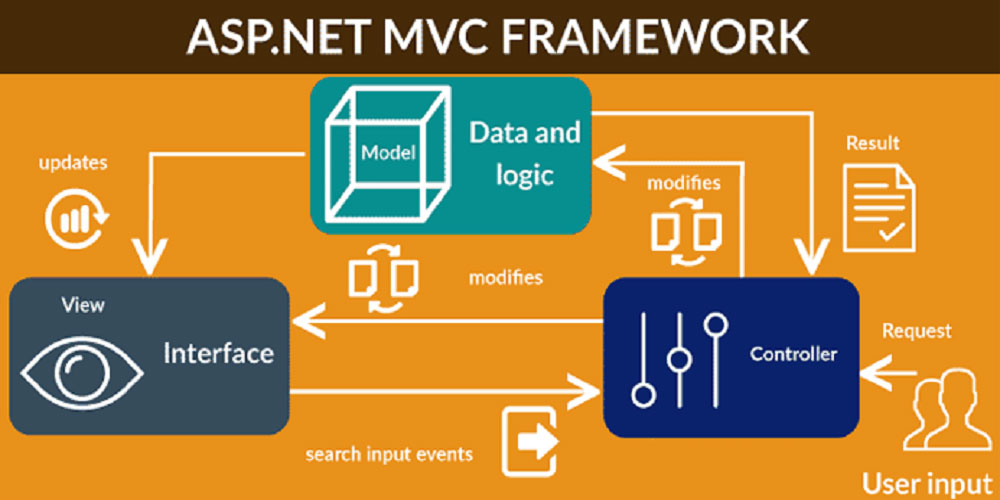
\includegraphics[width=0.8\textwidth]{fig/dotnetMVC.jpg}
    \caption[Schema pattern MVC]{Grafico che descrive il pattern \emph{Model-View-Controller}}
\end{figure}
Il modello MVC in ASP.NET Core è progettato per creare applicazioni web basate su pagine multiple (\emph{Multi-Page-Application}), in cui ogni pagina viene generata dinamicamente dal server in risposta alle richieste HTTP del client. Quando un utente richiede una pagina, il controller corrispondente elabora la richiesta, interagisce con il modello per recuperare o aggiornare i dati necessari, e infine seleziona una view per generare il markup HTML da inviare al client come risposta.
Come detto, la forza di MVC risiede nella chiara separazione delle responsabilità tra i componenti: il Model è costituito da classi C\# \emph{plain} che rappresentano i dati e la logica di business; ogni View è descritta da un file Razor (\texttt{.cshtml}), in cui del codice C\# è \emph{embedded} nel markup HTML per definire la logica di presentazione dei dati forniti contestualmente alla richiesta HTTP; ogni Controller è una classe C\# che eredita da \texttt{Controller}(fornita dal template ASP.NET Core MVC) e contiene metodi pubblici (\emph{action method}s) per manipolare i dati relativi alle richieste HTTP, e utilizza astrazioni sintattiche che consentono di predisporre in maniera chiara e intuitiva le risposte da inviare al client, spesso in maniera trasparente dal routing e dall'organizzazione interna del progetto.
Il modello MVC è particolarmente adatto per applicazioni web che richiedono una struttura ben definita, con una chiara separazione tra logica di business e presentazione, e che beneficiano di un approccio basato su pagine multiple. Inoltre, MVC offre un'ampia gamma di funzionalità integrate, come il supporto per la validazione dei modelli, l'autenticazione e l'autorizzazione, la gestione degli errori e l'integrazione avanzata con strumenti di sviluppo come Entity Framework Core e Identity Server (entrambi adottati nel progetto di tirocinio e descritti in seguito).

Il modello \textbf{Razor Pages} costituisce una sorta di via di mezzo tra Blazor e MVC, combinando alcuni aspetti di entrambi i modelli per offrire un approccio più semplice e diretto alla creazione di pagine web dinamiche.
Razor Pages è progettato per creare applicazioni web basate su pagine multiple, similmente a MVC, ma la struttura proposta è più snella e meno formale.
Mentre in MVC modello, logica e presentazione sono separati in entità distinte, e in Blazor ogni componente incapsula tali aspetti in confezioni pronte all'uso, Razor Pages adotta un approccio ibrido.
Come in MVC, ogni pagina Razor è costituita da un file \texttt{.cshtml} che combina markup HTML e codice C\# per la presentazione. Stavolta, a esso è accoppiato un \emph{Page Model}, un file di \emph{code-behind} (con estensione \texttt{.cshtml.cs}) che contiene la logica di gestione delle richieste, definendo metodi per ognuno dei verbi HTTP che si vogliono gestire.
Anche il routing è semplificato: ogni pagina Razor è automaticamente associata a un URL basato sulla sua posizione nella struttura del progetto, eliminando la necessità di definire esplicitamente le rotte come in MVC (ma perdendo al contempo della flessibilità garantita da una definizione esplicita).

In buona sostanza, la struttura a fondamento del modello Razor Pages è la stessa di MVC, ma vengono effettuate nette semplificazioni per ridurre la verbosità e la complessità del codice e il "lavoro di preparazione" \cite[p.28]{Pro_ASP.NET}, a scapito della flessibilità e della scalabilità. È una soluzione preferibile per applicazioni MPA di dimensioni medio-piccole, in cui la rapidità di sviluppo e la facilità di manutenzione sono prioritarie rispetto alla necessità di una struttura altamente modulare e scalabile.

L'ultima alternativa per la realizzazione di interfacce utente web con ASP.NET Core è l'adozione di framework JavaScript frontend per la creazione di \textbf{Single Page Application (SPA)}.
In questo scenario, ASP.NET Core funge da backend per definire la logica di backend, e il template appositamente fornito dal framework consente di associare tale logica a frontend JavaScript. I framework JavaScript con supporto maggiore per la realizzazione di SPA con backend .NET sono React, Angular e Vue, ognuno con le proprie caratteristiche e vantaggi.
Questa soluzione è adatta per team di sviluppo con competenze di frontend specifiche in JavaScript che non vogliono rinunciare alla potenza di un backend ASP.NET, o per progetti che richiedano un alto grado di interattività e reattività nell'interfaccia utente, sfruttando le potenzialità dei moderni framework JavaScript per creare esperienze utente fluide e dinamiche.

Il motivo per cui, nel contesto del progetto di tirocinio, si è scelto di adottare il modello MVC per la realizzazione della web app, anziché Blazor o Razor Pages, risiede principalmente nella maggiore maturità e stabilità del framework MVC, che vanta una lunga storia di utilizzo e supporto da parte della community. Questo aspetto è particolarmente rilevante in un contesto accademico, dove la solidità e l'affidabilità delle tecnologie adottate sono fondamentali per garantire il successo del progetto.
La maggiore modularità e scalabilità offerte dal modello MVC sono altresì cruciali per la gestione di un progetto, strutturato in un'architettura resiliente a microservizi, che renda più agevole la manutenzione e l'evoluzione dell'applicazione nel tempo.
L'altra motivazione cardine che ha portato alla scelta di MVC è la facilità d'integrazione: con alcuni potenti framework della piattaforma ASP.NET Core, quali Entity Framework Core e Duende Identity Server, (il modello MVC offre un'integrazione più diretta e completa, semplificando lo sviluppo e la gestione delle funzionalità di backend rispetto all'utilizzo di soluzioni differenti) e della soluzione MPA con strumenti di terze parti, poiché nell'ambito del fintech non è raro dover interagire con servizi legacy che, per garantire alti livelli di sicurezza e affidabilità, non possono essere facilmente sostituiti o aggiornati.

\section{SignalR}
SignalR è la libreria open source per Microsoft ASP.NET Core che consente di introdurre funzionalità real-time alle applicazioni web.
Questo prodotto consta sia di un package .NET server-side per fornire il servizio di notifica asincrona in tempo reale, sia una componente \emph{client-side} disponibile per più piattaforme (tra cui Javascript/Typescript per elevata compatibilità con i browser) che implementa la logica di \emph{subscription} al servizio di notifica.
L'astrazione proposta da SignalR è la seguente: il server ospita un \textbf{hub}, che rappresenta il "centro di smistamento" delle notifiche, e i client che desiderano instaurare una comunicazione bidirezionale real-time instaurano connessioni persistenti.
Il framework SignalR unisce una moltitudine di pattern di comunicazione, consentendo di scegliere l'approccio migliore per ogni necessità.
Per la comunicazione da client a server, l'hub consente di definire dei metodi che i client possono invocare da remoto, in puro stile \emph{RPC}; quando è il server a notificare i client, lo fa con un paradigma basato su messaggi in cui, specificando il metodo da invocare sui client e i target dell'invocazione, può passare i dati come parametri. Infatti, SignalR consente di suddividere i client connessi a un hub a diversi \textbf{groups}, permettendo così di aggregare con un solo metodo l'invocazione di tutti i client, uno solo o molteplici client appartenenti a una determinata categoria (consentendo di organizzare potenzialmente l'hub in pattern \emph{Pub/Sub}).

SignalR ricopre sostanzialmente tutti i casi in cui può essere necessaria una comunicazione real-time bidirezionale, specialmente nel caso di giochi, dashboard e tutte quelle applicazioni che richiedono uno scambio di informazioni continuo che genererebbe un overhead intollerabile affidandosi a normali richieste HTTP.
Ovviamente, il concetto di comunicazione asincrona in real-time non si inquadra bene nel contesto delle usuali richieste HTTP sincrone: SignalR introduce una catena di fallback che fornisce tre possibili implementazioni per la realizzazione di connessioni persistenti, applicando la soluzione percorribile (ossia possibile per il client) che garantisca performance più elevate.

Il sistema di trasporto più efficiente, ideale per la comunicazione con SignalR, è \textbf{WebSocket}: si tratta di un protocollo di rete che consente di instaurare una comunicazione \emph{full-duplex} su un'unica connessione TCP persistente. Il server SignalR elenca i tipi di trasporto consentiti, e se il client lo supporta, invia una GET HTTP per richiedere l'upgrade al protocollo WebSocket: in caso affermativo, viene instaurata una connessione TCP persistente che consente al server di inviare dati al client fin quando quest'ultimo resta connesso.
\begin{figure}[H]
    \centering
    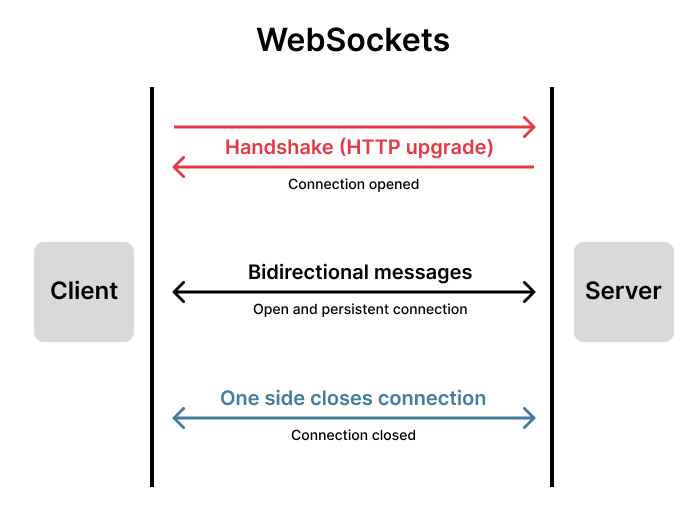
\includegraphics[width=0.5\textwidth]{fig/websocket.png}
    \caption[Diagramma Web Socket]{Fasi di una comunicazione bidirezionale mediante \emph{WebSocket}}
\end{figure}

In caso WebSocket non sia disponibile, l'alternativa più performante è \emph{Server-Sent Events} (\emph{SSE}), una tecnologia \emph{server push} che consente a un server di inviare dati al client in uno stream real-time unidirezionale ottenuto sulla base di un'unica richiesta HTTP la cui risposta "non termina" finché uno dei due capi non interrompe la connessione.
Questa alternativa è valida in casi in cui la necessità di una comunicazione real-time dipende dagli aggiornamenti del server al client: la performance in questa direzione è elevata, mentre la comunicazione SignalR da client a server prevede l'utilizzo di convenzionali richieste \emph{POST} HTTP, il cui overhead non consente una comunicazione fluida.
\begin{figure}[H]
    \centering
    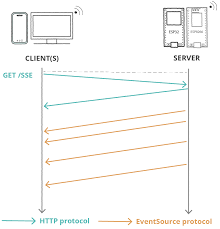
\includegraphics[width=0.4\textwidth]{fig/sse.png}
    \caption[Diagramma SSE]{Andamento di una comunicazione di tipo \emph{Server-Sent Events}}
\end{figure}

L'ultima tecnica utilizzata, in assenza delle due sopra descritte, è il \emph{Long Polling}: forte soltanto di HTTP e senza l'impiego di tecnologie aggiuntive, il client invia una richiesta al server, che mantiene "aperta" finché il server non ha un messaggio da inviare; quando al server arriva un aggiornamento, lo inoltra al client come risposta a tale richiesta; il client riceve la notifica, e ne invia immediatamente un'altra, che consentirà al server di inviare il prossimo aggiornamento non appena questo sarà disponibile. Tale approccio è universalmente adottabile da qualsiasi dispositivo che utilizzi HTTP versione 1.1 o superiore, ma costituisce la soluzione meno efficiente, con una performance peggiore dei SSE in comunicazione server-client, e pari a esso (richieste \emph{POST}) in comunicazione client-server.
\begin{figure}[H]
    \centering
    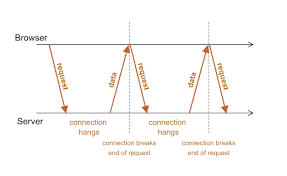
\includegraphics[width=0.6\textwidth]{fig/long_polling.png}
    \caption[Diagramma Long Polling]{Andamento di una comunicazione HTTP che realizza un \emph{long polling}}
\end{figure}

